\documentclass[a4paper]{article}
\usepackage[top=1.5cm, bottom=1.5cm, left=1.5cm, right=1.5cm]{geometry}
\usepackage[pdftex]{graphicx}
\usepackage{lscape}
\usepackage{pdflscape}

\newcommand{\tab}{\hspace*{1.5em}}
\setlength{\parskip}{7pt}

\begin{document}

\begin{titlepage}



\begin{center}

{\vspace*{8.5cm}}

% Upper part of the page


\textsc{\LARGE University of Aberystwyth}\\[1.5cm]

\textsc{\Large First year group project}\\[0.5cm]


% Title
\HRule \\[0.4cm]
{ \huge \bfseries UML2 Java}\\[0.4cm]

\HRule \\[1.5cm]

% Author and supervisor
\begin{minipage}{0.4\textwidth}
\begin{center} \large
\emph{Authors:}\\
Daniel Mal\'{y},\\ Samuel Sherar,\\ Lee Smith
\end{center}
\end{minipage}

\vfill


\end{center}

\end{titlepage}

\newpage
\tableofcontents 
\newpage

\section{Analysis}
	
\tab For our group project, we are required to design and implement a program that can create and convert Unified Modelling Language (UML) class diagrams to java stub code. For this we will create a graphical user interface, in which the user will be able to create, delete and modify classes, add relationships between classes and add text labels in a UML class diagram. 

The functionality of the program that we will implement can be split into three general groups: file management, software design and diagram editing. A use case diagram for each of the above groups is provided is provided below. 

\vspace{-10pt}
\begin{center}
	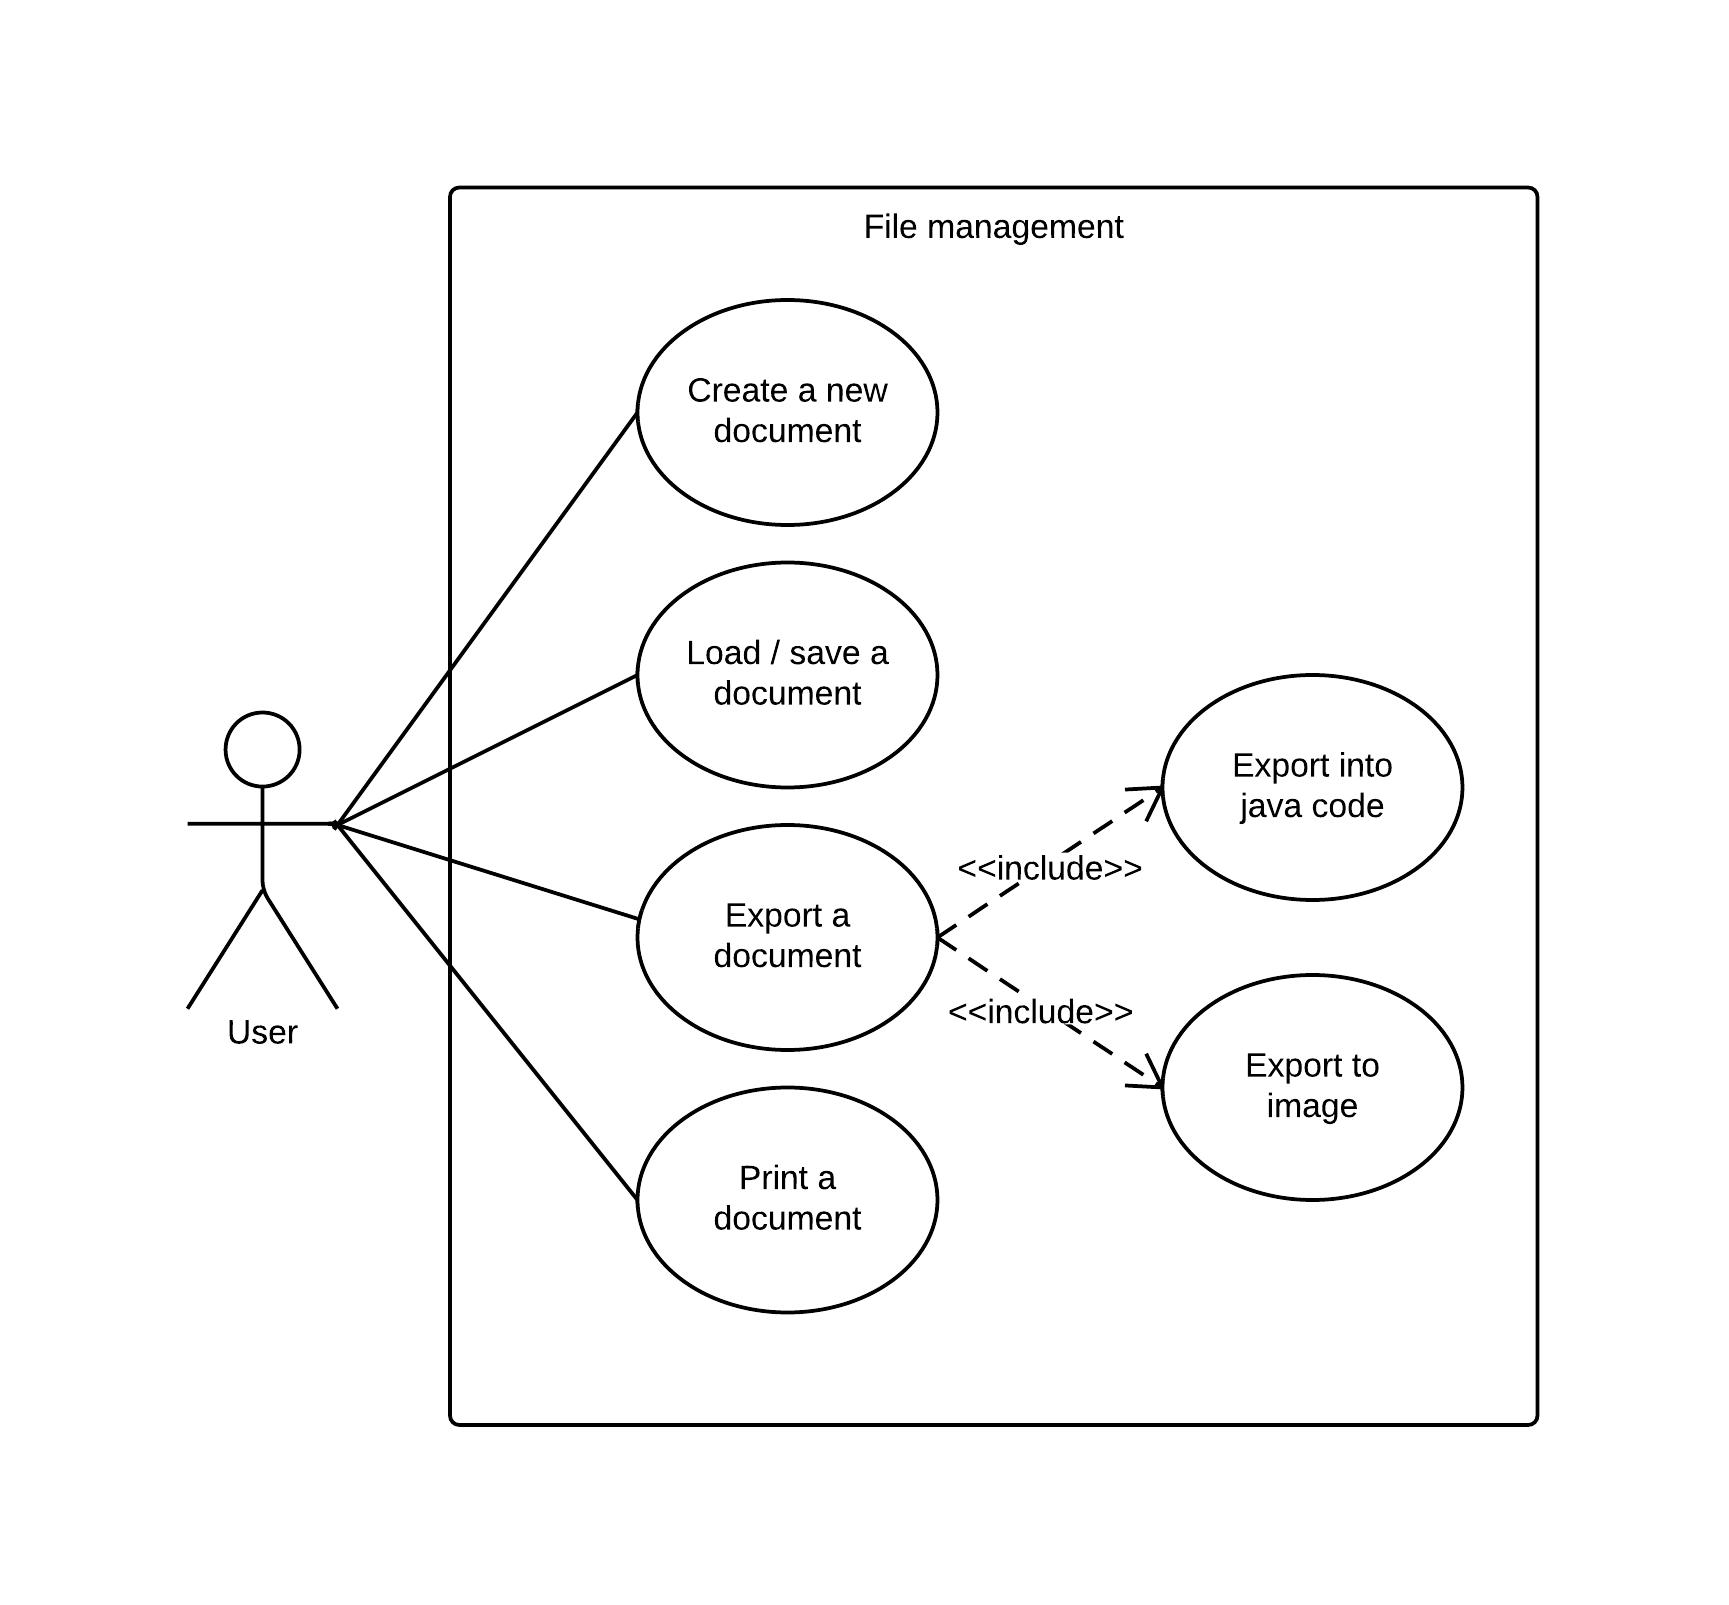
\includegraphics[trim=0 20pt 0 20pt,clip, width=0.8\textwidth]{FileManagementUseCaseDiagram.jpeg}
\end{center}
\vspace{-10pt}

The file management functionality of the program will include the following features: the user will be able to open a new document or load an existing one from a file, as well as save the current document. The program will also be able to export the currently opened class diagram into corresponding .java files containing the user-entered data fields and method stubs. It will also be possible to export a .png, .jpg or .gif image of the diagram canvas that can be easily added to any design documentation. The choice of file or directory relevant to each of these features will be up to the user and will be facilitated by the GUI. An option to print the current diagram will also be implemented.
 
%software design use case with caption

The software design features will include the following: creating a new class, adding data fields and methods to it using standard UML notation from which the program will automatically deduce certain parameters like visibility, type and so on. Modifiers that are not supported by direct UML notation will be accessible through a right-click menu, both for classes and for attributes. The user will be able to add relationships between classes, change their type and add labels and/or cardinalities to them. Any element created this way will be easily editable and removable.

%diagram editing use case with caption

As we are aiming to let the user produce complete UML class diagrams, additional features will be necessary. Class rectangles will be movable and resizable and the user will be able to add text labels to any point on the diagram. Relationships will be highly controllable: moving around points will be possible, as well as adding new points or removing existing ones. The canvas size will be configurable to allow facilitate image export and printing. The user will be able to change the global font used in the diagram and also view the diagram under zoom. We will also attempt to implement an undo / redo facility for user actions.

\section{Design}
	\subsection{Use-case Diagrams}
		% \input{./usecase.tex}
	\subsection{Class Diagrams}
		% \input{./classdiagram.tex}
	\subsection{Class Descriptions}
		\subsubsection{Model}
			
\tab The classes in the model package are designed to hold all the relevant data about a
document. When saving files, the model is all that is saved and it is all that is
necessary to then completely reconstruct the whole document. A document, that is a
user-created class diagram, is represented by the DocumentModel class. 
	
\paragraph{\small{\tab DocumentModel and DocumentPreferences\\*}}

\hspace{-10pt}The classes in the model package are designed to hold all the relevant data about a
document. When saving files, the model is all that is saved and it is all that is
necessary to then completely reconstruct the whole document. A document, that is a
user-created class diagram, is represented by the DocumentModel class. 
		\subsubsection{View}
			% \tab Each top-level model element (ClassModel, Relationship, TextLabelModel) has an associated view class: \textbf{ClassRectangle}, \textbf{RelationshipArrow} or \textbf{LabelView}, respectively. These all act as Observers to their associated models. They all contain methods that relate to painting and laying out the elements on the canvas. They also perform some controller duties, mainly while loading an existing document from a file and when adding sub-elements to their model as model classes cannot do this themselves.  All three inherit from the abstract class \textbf{DocumentElementView} which extends JPanel. This lets views be added to the diagram canvas as regular components. More information about what these classes do when the program runs can be found in descriptions of the implementation of individual use cases.

\paragraph{\small{\tab Diagram Layout\\*}}

\hspace{-10px}We actually had to define our own LayoutManager for the task of laying out components on the canvas. DiagramLayout works very similarly to absolute positioning . it polls the preferred size and location of the component in question and simply obeys its wishes.  No other LayoutManager in the Java API was appropriate for this task, however.

\paragraph{\small{\tab Geometry aides: Vector2D and RelationshipEndPoint\\*}}

\hspace{-10px}The Vector2D class is used heavily where relationships are concerned . we are not dealing with rectangular shapes anymore but lines. This requires some rather complicated geometry which would be impossible without the use of vectors. The RelationshipEndPoint class restricts the movability of java.awt.Point so that the endpoints of a relationship are unable to leave their assigned class rectangle. 

		\subsubsection{GUI}
			% \tab The GUI package manages the overall layout of the program, without interfering with the backend. All events triggered by the GUI.s elements are handled by the Manager class. 

		\subsubsection{Controller}
			% \paragraph{\small{\tab The multi-listener adapter: DiagramListener\\*}}

\hspace{-10pt}Due to the huge amount of methods listeners have to implement that we don.t always want, we defined our own adapter class implementing KeyListener, MouseMotionListener and MouseListener. Listeners extending this class will override only those methods that are relevant to their operation.

\paragraph{\small{\tab The controller triad: ClassController, LabelController, RelationshipController\\*}}

\hspace{-10pt}As with views, each of the three controllers has an associated model class. The controllers are added to views as listeners and when events happen on the views (such as the user clicking on a menu item in the right-click popup menu), they call the appropriate model methods. The controllers cannot access views directly . every single user action has to go straight through the model. Views are then updated in the usual Observable-Observer way. This ensures no user actions are .lost. in the views but it does require some additional overhead when the user requests the addition of a sub-element that only the view can perform. Methods in the model starting with .request.. are parts of this overhead.

\paragraph{\small{\tab Manager \\* }}

\hspace{-10pt}Originally, the Manager class was meant to be the only controller in the program. As the program grew, many of its duties had to be delegated to the elements themselves to avoid it growing into ridiculous size. It still retains, however, the task of listening to all of the events that occur in the GUI classes.  These events are interpreted and appropriate methods are called. In general, the Manager controls anything that is global to the current document. It also manages adding top-level elements to the document. The heart of the undo functionality also resides in the Manager as undos must be global to the document. 

\paragraph{\small{\tab ListeningMode: Turning a deaf ear on unwanted events\\*}}

\hspace{-10pt}A controller will not always want to react to events in the same way. The ListeningMode enum defines possible states in which a controller might be. Events will then be reacted to according to the mode currently set on the controller. 


		\subsubsection{Edit}
			% \tab The classes in the undo package closely follow the Java API specification for in-built undo support. Each of these classes represents a type of undoable edit. The edits store information about the former state and the latter state of an object and toggle between the states as requested by the user. The undo manager, the Manager class in our case, stores these edits and calls their undo() or redo() methods as needed (this is implemented in javax.swing.UndoManager which our Manager class extends). This architecture is based on the Commander design pattern. The presentation name attribute of these edits is used to update the status bar at the bottom of the application window.



		\subsubsection{Exporter}
			% \input{./exporterDesc.tex}
	\subsection{Algorithm Descriptions}
		\subsubsection{File Management Use Cases}
			% \paragraph{\small{\tab Creating a new document\\*}}

\hspace{-10pt}The command to open a new blank document is issued from the menu bar or when the application is launched. When the user clicks the appropriate menu item, the event gets sent to the Manager which calls its own openNewDocument() method. If any unsaved, user-initiated actions have been performed on the current document, a .do you want to save?. dialog appears. If the operation isn.t cancelled by the user (possibly after having saved), the canvas is emptied, the current DocumentModel loaded in the Manager is disposed of in favour of a new one, all undoable edits are discarded and new DocumentPreferences are set into the DocumentModel. Finally, the status bar is updated.

\paragraph{\small{\tab Saving a document\\*}}

\hspace{-10pt} Again, the command to save a document is initiated in the menu bar. Depending on the exact menu item clicked, save() or saveAs() is called in the Manager. If a filename is not associated with the document in the DocumentPreferences object, saveAs() is called anyway. This method brings up a JFileChooser letting the user select where the document should be saved to. Once a filename is obtained, serialize() is called and the DocumentModel currently in the Manager is simply written to that file using default Java serialization.

\paragraph{\small{\tab Loading a document from a file\\*}}

\hspace{-10pt} Loading a document is slightly trickier. We need to recreate views and controllers for all model objects and couple Observable-Observer pairs properly. When the command is issued by the user, the openExisting() method is called in the Manager. First, we need to dispose of the current document (see [section number] Creating a new document). The second stage is simply reading the DocumentModel object from the file the user selected (again by means of a JFileChooser). It is loaded into the Manager which then: calls cleanUp() on the DocumentModel which will cause it to discard all non-existent elements, calls getView() on each DocumentElementModel, adds the returned DocumentElementViews to the Canvas, ties up Observers with Observables, reads DocumentPreferences on the loaded object and sets the document properties accordingly. The individual DocumentElementView constructors do very much the same for sub-elements (e.g. views are created and added for Attributes and so on). They also create and assign controllers.

\paragraph{\small{\tab Exporting a document\\*}}

\hspace{-10pt}Exporting to code can be triggered from two locations, either from the MenuBar under Export or from the SideBar under .Export to Java... This calls the Exporter constructor using DocumentModel that contains all the objects and information needed to create the code. Within the Exporter class there are five private methods which will create the code sections, createClassFileContents(), which pulls the following four methods together into one string to be used within the exportCode() method. getHeaderString() creates the class header along with any classes that will be extended or implemented, getAttributeString() will take all the variables written into the class to be created, get the visibility, name, type and any modifiers that will be added to it. getCardinalitiesString(),  depending on the type of cardinalities and relationships, will create fixed or open arrays or ArrayLists, respectively with the ClassName as the type. getMethodsString() will take methods that the user enters, again taking visibility, name, any parameters and their types, and the return type of the method. The exportCode() method will then run through an ArrayList of all the filenames and Strings created and output each file as a .java filetype. The selection of output directory is facilitated by a JFileChooser.

\paragraph{\small{\tab Exporting to an image\\*}}

\hspace{-10pt}Another Exporter Constructor will take the canvas and render it into a BufferedImage, and create a graphic from this. A JFileChooser will allow the user to change the image type of .png, .gif or .jpg. and save the file accordingly.

\paragraph{\small{\tab Printing a Diagram\\*}}

\hspace{-10pt} This will be fairly similar to exporting an image, using the canvas a Constructor parameter. A print() method will again create a graphic to be used, but will be scaled depending on the default paper size from PageFormat before printing to the selected printer.


		\subsubsection{Software Design Use Cases}
			% \paragraph{\small{\tab Creating a class (includes setting class name)\\* }}

\hspace{-10pt} When the .New Class. button is clicked on the side bar, the Manager receives the event and sets ListeningMode.PLACING\_CLASS on itself. The coordinates of the next mouse event that will be received from the canvas will be sent to the addNewClass() method in the Manager. This method resets the listening mode, creates a new ClassModel, assigns a view (ClassRectangle) to it, bootstraps Observer-Observable pairs and adds the view to the canvas. It also creates a new ExistenceEdit holding the new ClassModel (more on undoable edits in the section about undo functionality). As soon as the class is created, the TextLabelModel that acts as the name label is asked to enable editing on itself so the user can type in the name of the class immediately (this happens in the ClassRectangle constructor which also creates and assigns a ClassController).

\paragraph{\small{\tab Adding attributes to a class\\*}}

\hspace{-10pt} This use case is not handled by the Manager as the request does not come from the GUI or the canvas. The request to add a new attribute comes from a class rectangle right-click menu and so the appropriate ClassController will receive the event. The ClassController then calls requestNewDataField() or requestNewMethod(), as appropriate and the ClassModel.s view (ClassRectangle) is notified. addAttributeToModel() is called in the ClassRectangle which creates the Attribute object, assigns a LabelView object to it, adds the LabelView to itself, adds the Attribute to the ClassModel , couples the Attribute with the LabelView and immediately enables editing on the new Attribute. An ExistenceEdit is also created and sent to the Manager.

\paragraph{\small{\tab Behind the scenes: Derive attributes from UML representation\\*}}

\hspace{-10pt}Instead of using standard String manipulations, we decided to match them against a Regex pattern, as some people enter UML notation differently and a lot of the notation is not mandatory. Therefore we created 3 different Regular Expressions: one for matching Data fields; another for the .shell. of the method (the method without any parameters); and finally one for the method parameters. Then using Java.s incredibly powerful Regex engine, which automatically splits the up the matched string into specified groups, we can individually pull out parts of the string to test them against UML patterns and set the variables accordingly. If the Attribute representation doesn.t conform to UML, the whole Attribute is flagged as invalid.

\paragraph{\small{\tab Editing modifiers and flags\\*}}

\hspace{-10pt}Modifiers and flags can be set or unset through right-click menus on class rectangles or attributes. The appropriate ClassController (or LabelController for Attributes) receives the event, sets the appropriate modifier or flag (or combination thereof) by calling a setter in the model. This creates a FlagEdit and sends it to the Manager. The font style is overridden accordingly on the name label of the class or on the attribute string, whichever is applicable.

\paragraph{\small{\tab Adding relationships\\*}}

\hspace{-10pt}Adding a relationship between two classes is a three-stage process. It can be triggered either from the sidebar or from a class right-click menu. Either way, the Manager (which implements Observer only for this purpose) receives the request and sets ListeningMode.PLACING\_RELATIONSHIP on itself. If the request comes from a class, that ClassModel is added to the selectionStack in the Manager. If it comes from the sidebar, addNewRelationship() with no arguments is called in the Manager. The Manager will now listen to changes in the paint state of ClassModels. Once any one ClassModel passes into SELECTED state (as set by a ClassController), it is added to the selectionStack and from this point, both ways of the process follow the same path. The listening mode does not change, and the Manager waits for a second class to be selected. Once that happens, addNewRelationship() is called with both ClassModels and a new Relationship along with a RelationshipArrow is created in much the same way as a class.  Listening mode is set back to LISTEN\_TO\_ALL, the selectionStack is emptied and an ExistenceEdit is created.

\paragraph{\small{\tab Changing the relationship type\\*}}

\hspace{-10pt}The type of the relationship can be changed in the relationship right-click menu. The appropriate RelationshipController receives the event, creates a RelationshipStateEdit to store the current state of the Relationship and changes the type of the model. The view is then repainted.

\paragraph{\small{\tab Adding cardinalities / labels to relationships\\*}}

\hspace{-10pt} See section on adding Attributes to ClassModels. The process of adding sub-elements to Relationships follows exactly the same process, especially since Attribute, Cardinality and RelationshipLabel all inherit from TextLabelModel.

\paragraph{\small{\tab Removing elements \\*}}

\hspace{-10pt}Removing elements is simple. A class or a relationship may only be removed through the right-click menu but any textual element may also be removed by deleting all text and pressing ENTER. Both produce the same result . the userRemove() method is called on the appropriate DocumentElementModel which sets the .exists. variable to false and creates an ExistenceEdit, sending it to the Manager. Observers are notified and when a view learns that its model has been removed, it sets itself to invisible, removes itself from the parent container but keeps a reference to it in the .suspendedParent. variable. It is important to note that the whole MVC triad of the element remains in the program and the DocumentElementModel remains in the document until cleanUp() is called on DocumentModel. This is so that undoing a remove can easily bring back an element into existence. 

\paragraph{\small{\tab Editing textual elements\\*}}

\hspace{-10pt} Whenever the user double-clicks a LabelView, the LabelController will set editing to true in the model. Through update(), this will call enableEdit() in LabelView. This method removes the whole view from its parent, replaces it with a JTextArea at the same location, requests immediate focus for the JTextArea and selects all the text within it. The LabelController assigned to this LabelView will now listen to the JTextArea as well. Once the user presses ENTER, this process is rolled back by the exitEdit() method. The text of the label is set to the text of the JTextArea and the label is re-added to the parent component. Also, a TextEdit is created and sent to the Manager. If no text is in the JTextArea as it is validated, the model is userRemove().d.

		\subsubsection{Diagram Editing Use Cases}
			%\paragraph{\small{\tab Moving and resizing class rectangles\\*}}

\hspace{-10pt}Moving class rectangles is simple enough. Whenever the mouse is dragged on a ClassRectangle component, the ClassController updates the location of the ClassModel which then notifies its observers. A LocationEdit is created and sent to the compoundEdit residing in the ClassModel. Once dragging is finished, the whole compound edit is sent to the Manager. The ClassRectangle changes its own location in accordance and the Canvas is forced to re-layout. However, we need to think about Relationships as well. This is where the RelationshipEndPoint class comes in. Each RelationshipEndPoint is defined as having a precise position on the border of the class rectangle. When this changes its (x,y) coordinates, the (x,y) coordinates of the RelationshipEndPoints can be updated easily as well. For this reason, Relationships implement Observer. Whenever a ClassModel changes location, the new location is passed to RelationshipEndPoints through the update() method in Relationship. The endpoints are then forced to update their coordinates to the new rectangle.  
Resizing class rectangles works in a similar way. Whenever the user mouses over the bottom-right corner of the class rectangle, the cursor is set to system default resize cursor and the element paint state is set to MOUSED\_OVER\_RESIZE. While this paint state is set, any dragging motion will result in the class rectangle being resized.  The rest of the process follows that of moving class rectangles, except instead of LocationEdits, SizeEdits are being created. 

\paragraph{\small{\tab Text labels outside any other element\\*}}

\hspace{-10pt}Adding explanatory text labels to a class diagram is a useful feature. It is implemented by simply creating a new TextLabelModel from the Manager (in much the same way as any other element). Please refer to the section on modifying textual elements . free labels adhere to this model. 

\paragraph{\small{\tab Controlling relationship arrows\\*}}

\hspace{-10pt} Relationship arrows only receive mouse events when the mouse is actually on the arrow, even though the actual component size is many times larger. This is done by overloading the contains(Point) method (for further details on this method, please refer to the javadoc). Whenever the user clicks on a point that is already present in the ArrayList of Points in the Relationship object, the Point can be moved around. If this point is an endpoint and therefore attached to a class rectangle, the overloaded move(int, int) method in RelationshipEndPoint ensures it stays there. If a user clicks and drags somewhere else, a new point is added to the line. The addPoint() method is called in Relationship. It checks all the existing segments and determines to which one the new point should belong. It then inserts the Point object into the ArrayList at the appropriate index. Removing a point is done by double-clicking on it. The RelationshipController simply calls removePoint() with the mouse event coordinates and the method determines whether a point should be removed, and if so, which one. Updating the view is done in the usual way.
Moving labels and cardinalities on Relationships works the same way as moving any other element. The only difference is that the movement is restricted . a Cardinality may never be further than a certain distance from its associated endpoint. Similarly, a RelationshipLabel cannot leave its Relationship. This constraint must be enforced not only for user actions but also for when relationships move as a result of something else moving. For this reason, Cardinalities and RelationshipLabels both have a fixed relative position to a reference point on the relationship arrow. When this reference point moves, realign() methods are called in the sub-elements and these reposition themselves. This way, a relationship cannot .run away. from its cardinalities.

\vspace{-5pt}\paragraph{\small{\tab Undo and redo functionality\\*}}

\hspace{-10pt} The undo functionality in the application is built atop the Java UndoManager framework. The Manager class extends UndoManager which, in turn, implements UndoableEditListener. DocumentElementModel has an addUndoableEditListener() method through which the Manager is assigned as a destination for UndoableEditEvents  to each and every element. Whenever a user-initiated action is acted upon, an UndoableEdit is created and sent to the fireUndoableEvent() method in DocumentElementModel. This method wraps the edit in an event and sends it to the Manager. From there on, undoing is defined by the Java API. Our undo package defines six types of UndoableEdits, all extending the AbstractUndoableEdit class. All of these store information about the previous state and the current state of the model object in question and override the undo() and redo() methods, toggling the states as needed. 

\emph{A note on existence.} As removed objects stick around in the program, it is relatively easy to bring them back into existence using the resurrect() method defined in DocumentElementModel. They can also be removed again, this time by using remove(). However, once cleanUp() is called on DocumentModel, they disappear from it. Trying to undo removes after that might still work but will create unpredictable behaviour when saving is thrown into the mix. When a document is exported into java code, it is cleaned up as we don.t want removed elements to appear in the actual code. This is why exporting disables all undos and redos on edits created before exporting was initiated. This is clearly a bug in the application, albeit forced, and we will be looking to fix it in the future. 

\emph{A note on relationship states.} Undoing actions on relationships works slightly differently than the other edits. In order to avoid having to create lots of edit classes for the many operations relationships allow to be performed on them, a whole relationship is simply cloned into a RelationshipStateEdit. When undoing, the current object simply copies all of its data from the cloned previous version.  

\vspace{-5pt}\paragraph{\small{\tab Resizing the canvas\\*}}

\hspace{-10pt} The Canvas is contained in a JPanel that has DiagramLayout set on it. This means that it will respect the canvas. preferred size no matter what it may be. It allows us to let the user resize the canvas to his liking. A canvas can either be snapped to the minimum size to contain all of its components through the fitToDiagram() method in the Manager or a resize dialog can be thrown up to let the user specify an exact size in pixels. This is implemented in the resizeCanvasDialog() function in the Manager and a separate ResizeDialog class.  The workings of this functionality are trivial. More information on it may be found in the javadoc. 


\vspace{-5pt}\paragraph{\small{\tab Changing the font\\*}}

\hspace{-10pt}When the user changes the font name or the font size on the toolbar, the changeFont() method is called in the Manager. This method simply sets the new font into DocumentPreferences and it is up to the Observers of DocumentPreferences to set their own font accordingly. Each top-level element has a clause in the update() method that lets them respond to changes in font. Also, top-level elements have to force their own font into their sub-elements by directly calling their setFont() method.

\vspace{-5pt}\paragraph{\small{\tab Changing the zoom\\*}}

\hspace{-10pt}This is a feature that was partially implemented at the very early stages of development. As the program grew, the support for the zoom feature throughout the program waned and it was decided that it would be completed later on. However, due to time constraints, this .later on. never materialized as implementing zoom got eclipsed by much more important features to implement and debug, such as undos. Completing the zoom may or may not be very difficult; however, there just wasn.t enough time to try it out. The zoom slider in the GUI is intentionally disabled and all methods relating to zoom are currently deprecated throughout the code. We are planning on fixing this in the future.

	 
 \begin{landscape}
\section{Testing}
\begin{tabular}{| p{3cm} | p{7cm} | p{7cm} | p{6cm} | }
	\hline
	Test Done & Expected Result & Actual Result & Comments \\ \hline
	Adding class & Class drawn on the canvas & What was expected & \\ \hline
	Zooming the elements & When zoomed, relational spacing keeps the same and everything still keeps functionality & Nothing is editable, but relational space between elements are correct & Will be fixed later before released \\ \hline
\end{tabular}

 \end{landscape}
\newpage
%Hello World!

\section{Evaluation}
	% \input{./evaluation.tex}
\end{document}
